\chapter{Результаты: механизмы сосуществования}

\section{Механизмы сосуществования в пространствах различных рамерностей}

В рамках нашего исследования предложено исследовать равновесные положения популяции в пространстве параметров модели, описанном выше, с ограничениями на некоторое подмножество параметров, которые приводит к нетривиальным стационарным точкам системы; такие ограничения также известны как \textit{механизмы сосуществования}, поскольку отсутствие нулевых стационарных решений есть выживание всех видов популяции.

\subsection{Competition-colonization trade-off}

В данной части работы мы приведем более точные иллюстрации для наблюдаемой реализации широко известного механизма \textbf{competition-colonization trade-off}; биологическое соображение, описывающее данный механизм, заключается в том, что сосуществование двух видов возможно, если один из видов сильнее конкурирует, а второй распространяется на большие расстояния, что в нашем пространстве можно наблюдать в пространстве $ \left[\sigma_{m2};\;d'_{12}\right] $, где $\sigma_{m2}$ есть дисперсия ядра рождения второго вида (т.е. его радиус распространения), а $d'_{12}$ --- агрегированная сила конкуренции со стороны 1-го вида на 2-ой . Несложно заметить, что данное соображение описывает равновесные устойчивые положения модели «хищник–жертва».

Главной целью нашего исследования являются эффекты увеличения размерности геометрического пространства, в котором обитают особи. Рисунки \ref{fig:cctod1}, \ref{fig:cctod2} and \ref{fig:cctod3} иллюстрируют случаи $ \mathbb{R}^{1} $, $ \mathbb{R}^{2} $ и $ \mathbb{R}^{3} $ соответственно. В рамках выполнения работы нами был разработан численный метод, позволяющий считать решения системы точнее, чем ранее известные методы за счет экспоненциальной скорости сходимости и уменьшения выполняемых арифметических операций, что не позволяет ошибке накапливаться. Для каждого случая приведены два графика: поверхности плотностей индивидов (первых моментов) для каждой пары параметров $ (\sigma_{2}^{m};d'_{12}) $ и области в пространстве параметров, которые индуцируют сосуществование или существование только одного из видов (номер выживающего вида подписан на рисунке).

Исходя из полученных результатов, необходимо сделать следующий набор выводов и подчеркнуть следующие особенности:

\begin{figure*}
	\centering
	\begin{subfigure}{.5\textwidth}
		\centering
		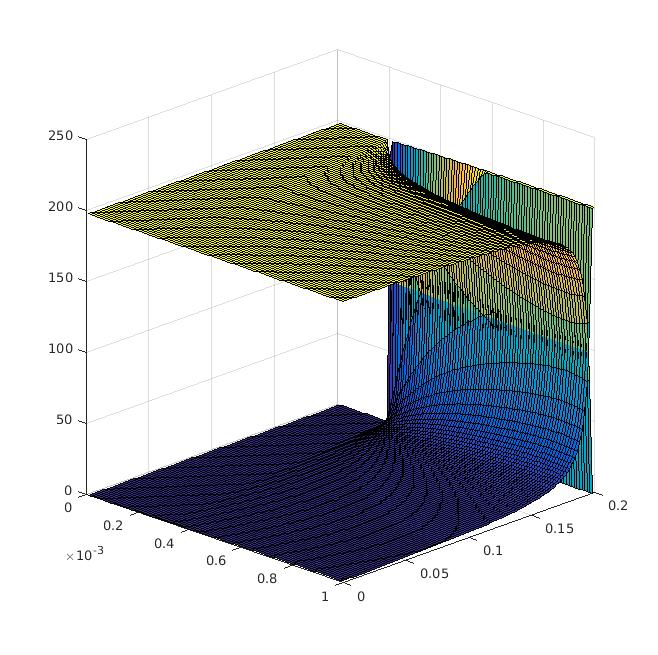
\includegraphics[width=.95\linewidth]{N1N2cctoD1.jpg}
		\caption{Поверхности первых моментов \(N_1\) и \(N_2\) в описанном пространстве параметров}
		\label{fig:cctod1:sub1}
	\end{subfigure}%
	\begin{subfigure}{.5\textwidth}
		\centering
		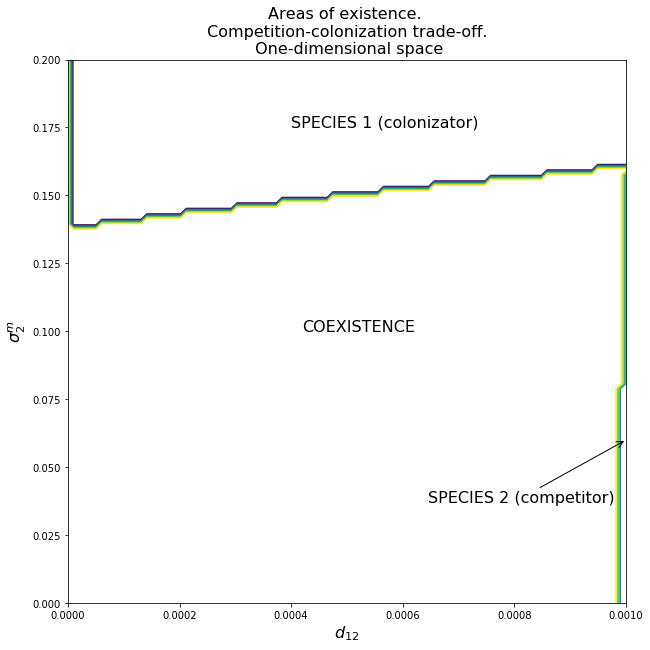
\includegraphics[width=.95\linewidth]{arccto08d1.png}
		\caption{Области сосуществования в описанном пространстве параметров} 
		\label{fig:cctod1:sub2}
	\end{subfigure}
	\begin{subfigure}{.5\textwidth}
		\centering
		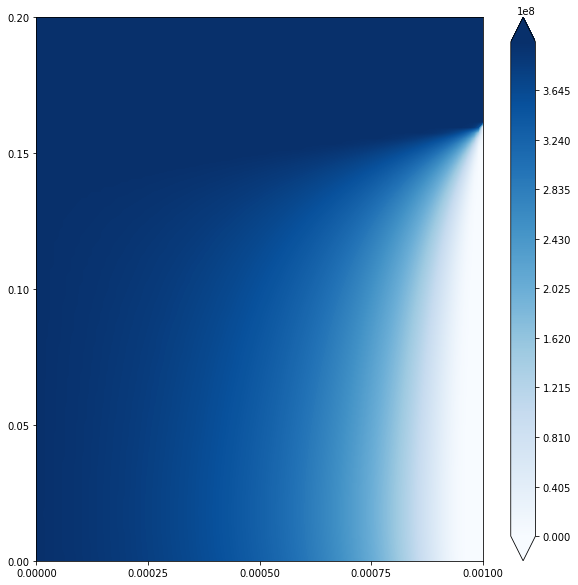
\includegraphics[width=.95\linewidth]{ccto_d1_n1.png}
		\caption{Heat map численности первого вида (colonizator) в описанном пространстве параметров}
		\label{fig:cctod1:sub3}
	\end{subfigure}%
	\begin{subfigure}{.5\textwidth}
		\centering
		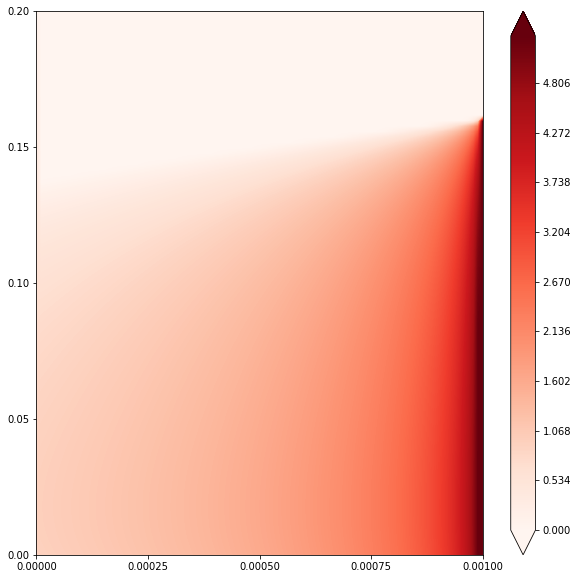
\includegraphics[width=.95\linewidth]{ccto_d1_n2.png}
		\caption{Heat map численности первого вида (competitor) в описанном пространстве параметров} 
		\label{fig:cctod1:sub4}
	\end{subfigure}
	\caption{Реализация механизма Competition-Colonization Trade-Off  в пространстве параметров  $\sigma^m_2$ и $d'_{12}$ в случае  \emph{одномерной области обитания}. Оставшиеся параметры выбраны следующим образом:  $b_{1}=b_{2}=0.4
		, d_{1}=d_{2}=0.2
		, d'_{11}=d'_{22}=d'_{21}=0.001,
		\sigma_{1}^{m}=0.04
		, \sigma_{11}^{w}=\sigma_{12}^{w}=\sigma_{21}^{w}=\sigma_{22}^{w}=0.04$}
	\label{fig:cctod1}
\end{figure*}

\begin{figure*}
	\centering
	\begin{subfigure}{.5\textwidth}
		\centering
		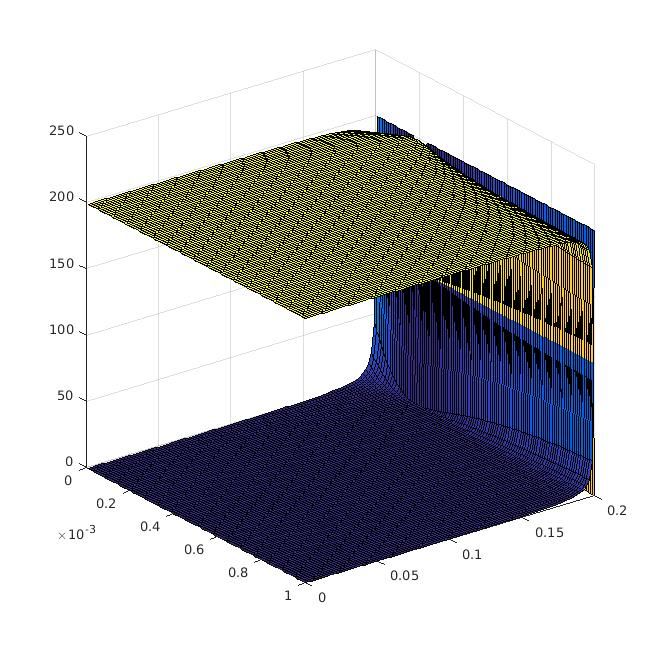
\includegraphics[width=.95\linewidth]{N1N2cctoD2.jpg}
		\caption{Поверхности первых моментов \(N_1\) и \(N_2\) в описанном пространстве параметров}
		\label{fig:cctod2:sub1}
	\end{subfigure}%
	\begin{subfigure}{.5\textwidth}
		\centering
		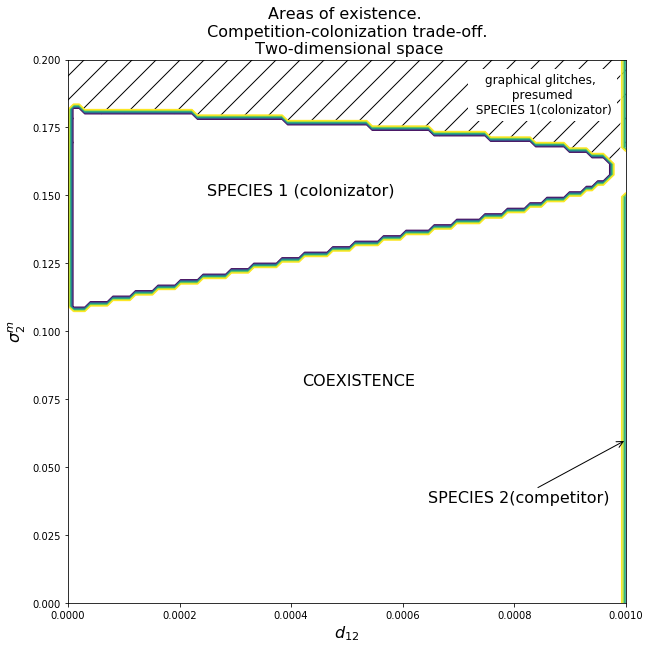
\includegraphics[width=.95\linewidth]{arccto08d2.png}
		\caption{Области сосуществования в описанном пространстве параметров}
		\label{fig:cctod2:sub2}
	\end{subfigure}
	\centering
	\begin{subfigure}{.5\textwidth}
		\centering
		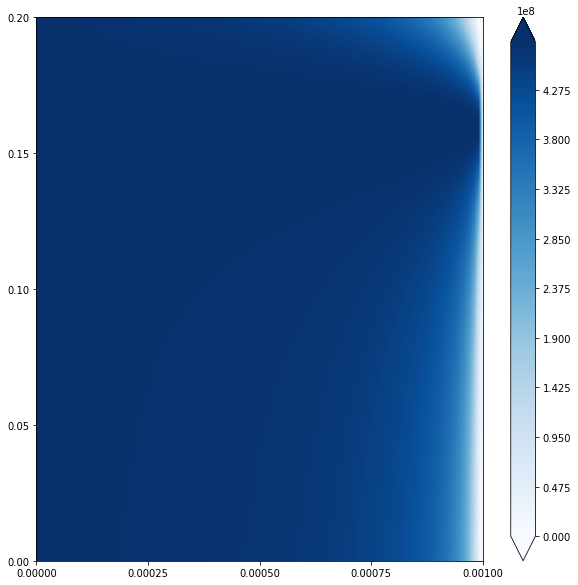
\includegraphics[width=.95\linewidth]{ccto_d2_n1.png}
		\caption{Heat map численности первого вида (colonizator) в описанном пространстве параметров}
		\label{fig:cctod2:sub3}
	\end{subfigure}%
	\begin{subfigure}{.5\textwidth}
		\centering
		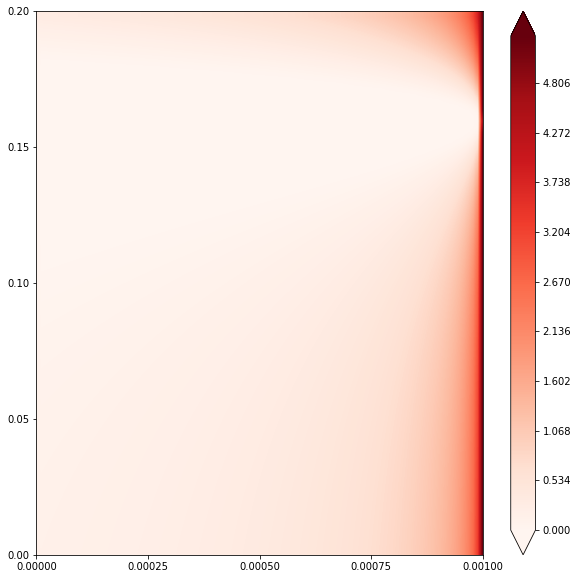
\includegraphics[width=.95\linewidth]{ccto_d2_n2.png}
		\caption{Heat map численности первого вида (competitor) в описанном пространстве параметров}
		\label{fig:cctod2:sub4}
	\end{subfigure}
	\caption{Реализация механизма Competition-Colonization Trade-Off  в пространстве параметров  $\sigma^m_2$ и $d'_{12}$ в случае  \emph{двумерной области обитания}. Оставшиеся параметры выбраны следующим образом:  $b_{1}=b_{2}=0.4
		, d_{1}=d_{2}=0.2
		, d'_{11}=d'_{22}=d'_{21}=0.001,
		\sigma_{1}^{m}=0.04
		, \sigma_{11}^{w}=\sigma_{12}^{w}=\sigma_{21}^{w}=\sigma_{22}^{w}=0.04$}
	\label{fig:cctod2}
\end{figure*}


\begin{figure*}
	\centering
	\begin{subfigure}{.5\textwidth}
		\centering
		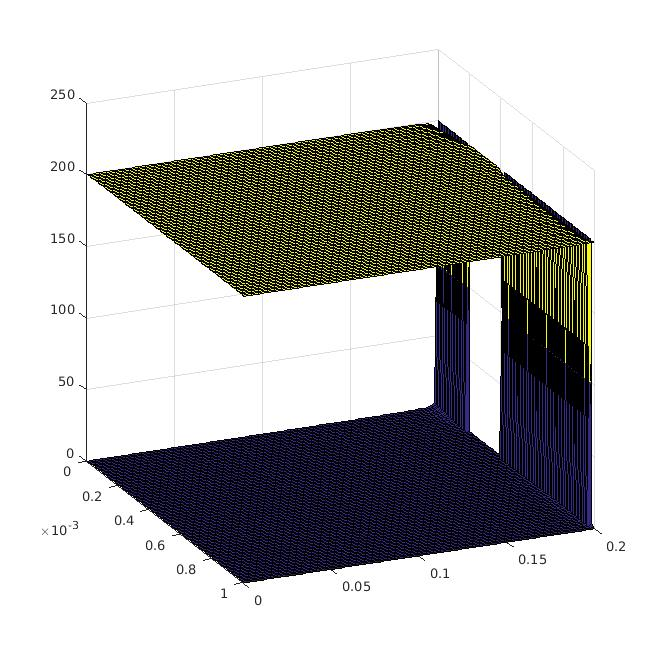
\includegraphics[width=.95\linewidth]{N1N2cctoD3.jpg}
		\caption{Поверхности первых моментов \(N_1\) и \(N_2\) в описанном пространстве параметров}
		\label{fig:cctod3:sub1}
	\end{subfigure}%
	\begin{subfigure}{.5\textwidth}
		\centering
		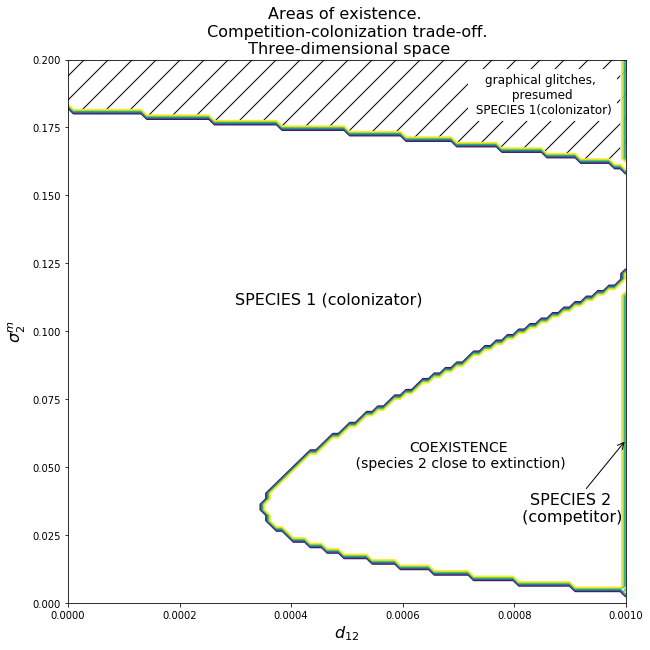
\includegraphics[width=.95\linewidth]{arccto08d3.png}
		\caption{Области сосуществования в описанном пространстве параметров}
		\label{fig:cctod3:sub2}
	\end{subfigure}
	\centering
	\begin{subfigure}{.5\textwidth}
		\centering
		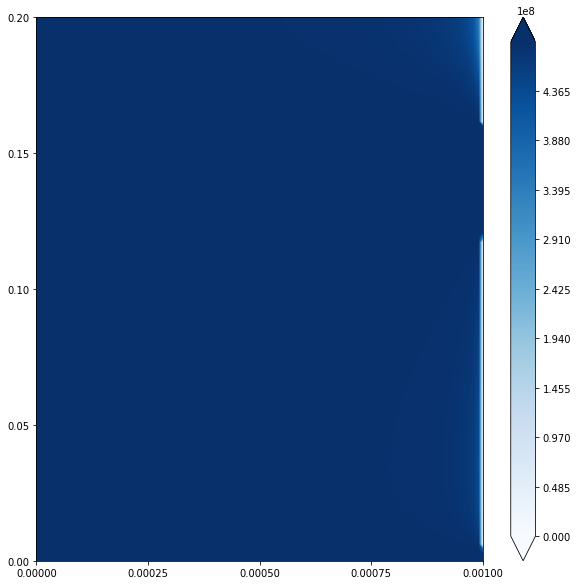
\includegraphics[width=.95\linewidth]{ccto_d3_n2.png}
		\caption{Heat map численности первого вида (colonizator) в описанном пространстве параметров}
		\label{fig:cctod3:sub3}
	\end{subfigure}%
	\begin{subfigure}{.5\textwidth}
		\centering
		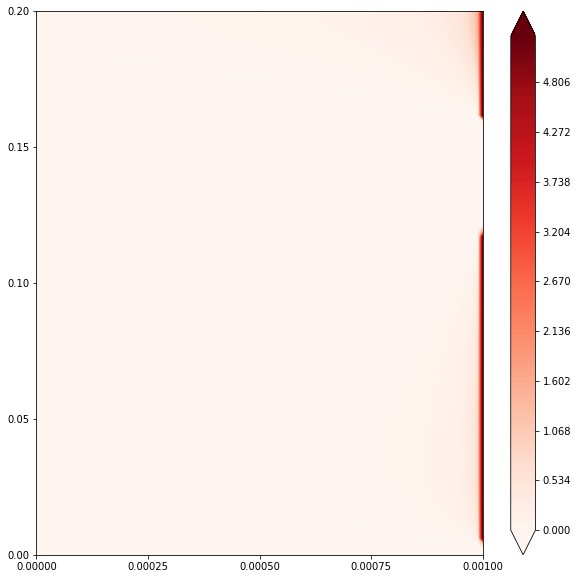
\includegraphics[width=.95\linewidth]{ccto_d3_n1.png}
		\caption{Heat map численности первого вида (competitor) в описанном пространстве параметров}
		\label{fig:cctod3:sub4}
	\end{subfigure}
	\caption{Реализация механизма Competition-Colonization Trade-Off  в пространстве параметров  $\sigma^m_2$ и $d'_{12}$ в случае  \emph{трехмерной области обитания}. Оставшиеся параметры выбраны следующим образом:  $b_{1}=b_{2}=0.4
		, d_{1}=d_{2}=0.2
		, d'_{11}=d'_{22}=d'_{21}=0.001,
		\sigma_{1}^{m}=0.04
		, \sigma_{11}^{w}=\sigma_{12}^{w}=\sigma_{21}^{w}=\sigma_{22}^{w}=0.04$}
	\label{fig:cctod3}
\end{figure*}


\begin{itemize}
	
	\item общая идея механизма competition-colonization trade-off наблюдается во всех трех размерностях; при этом механизм нельзя воспринимать, как правило, необходимо требующее для сосуществования двух видов перераспределения второго; как показано на наших рисунках, увеличение $ \sigma_{2}^{m} $ ведет к вымиранию сильного вида; 
	
	\item с ростом размерности геометрического пространства вид-колонизатор вытесняет более сильный вид и даже приводит к его вымиранию: общий тренд заключается в увеличении области выживания исключительно первого вида, в то время как область сосуществования двигается (двумерный случай) и уменьшается (трехмерный случай); 
	
	\item в трехмерном случае вид-колонизатор фактически приводит к вымиранию более сильного вида при всех рассмотренных наборах параметров модели; выделенная область сосуществования, несмотря на то, что оба вида там выживают, приводит к фактическому вымиранию более сильного вида, с резким ростом к границе области, где сильный вид выигрывает (рис. \ref{fig:cctod3:sub3}, \ref{fig:cctod3:sub4});
	
	\item как видно из рисунков \ref{fig:cctod2:sub2} и \ref{fig:cctod3:sub2} разработанный численный метод имеет несколько численных артефактов, которые можно устранить увеличением вычислительной точности нашего метода.
\end{itemize}



\subsection{Heteromyopia}

В данной части работы мы рассмотрим другой механизм сосуществования, который был предложен в \cite{MURRELL}, \textit{heteromyopia}: драйвером сосуществования в рамках данного механизма считается принцип о том, что межвидовая конкуренция индивидов проходит на меньшем расстоянии, чем внутривидовая. В нашей модели мы нашли данный механизм в пространстве параметров $ \left[\sigma_{ii}^{w};\sigma_{ij}^{w}\right] $ (т.е. в пространстве дисперсий ядер конкуренции).

Главной целью нашего исследования являются эффекты увеличения размерности геометрического пространства, в котором обитают особи. Рисунки \ref{fig:hmd1}, \ref{fig:hmd2} и \ref{fig:hmd3} иллюстрируют случаи $ \mathbb{R}^{1} $, $ \mathbb{R}^{2} $ и $ \mathbb{R}^{3} $ соответственно. В рамках выполнения работы нами был разработан численный метод, позволяющий считать решения системы точнее, чем ранее известные методы за счет экспоненциальной скорости сходимости и уменьшения выполняемых арифметических операций, что не позволяет ошибке накапливаться. Для каждого случая приведены два графика: поверхности плотностей индивидов (первых моментов) для каждой пары параметров $ \left[\sigma_{ii}^{w};\sigma_{ij}^{w}\right] $ и области в пространстве параметров, которые индуцируют сосуществование или существование только одного из видов (номер выживающего вида подписан на рисунке).

Исходя из полученных результатов, необходимо сделать следующий набор выводов и подчеркнуть следующие особенности:

\begin{itemize}
	\item в целом, корректность предложенного механизма была подтверждена в случае одномерного и трехмерного пространства обитания; стоит также отметить, что предложенная в оригинальной статье линейность зависимости между радиусом интравидовой и интервидовой конкуренции является неплохим, но не самым лучшим первым приближением; 
	
	\item описанный механизм отсутствует в случае двумерной среды обитания, что ставит вопросы о его значимости и корректности; 
	
	\item согласно рисункам \ref{fig:hmd1:sub2}, \ref{fig:hmd2:sub2} и \ref{fig:hmd3:sub2} разработанный численный метод, как и в случае рисунков для competition-colonization trade-off выше, содержит набор численных артефактов.
\end{itemize}

\begin{figure*}[ht]
	\centering
	\begin{subfigure}{.5\textwidth}
		\centering
		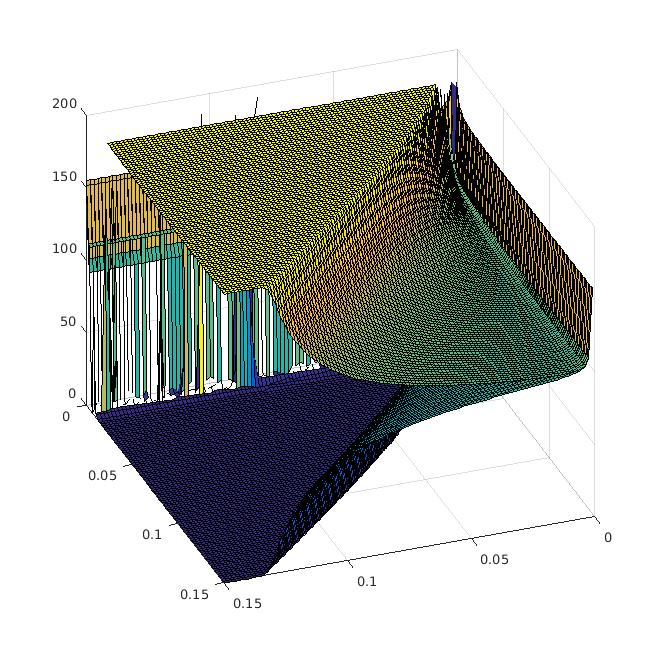
\includegraphics[width=.93\linewidth]{N1N2hm08D1.jpg}
		\caption{Поверхности первых моментов \(N_1\) и \(N_2\) в описанном пространстве параметров}
		\label{fig:hmd1:sub1}
	\end{subfigure}%
	\begin{subfigure}{.5\textwidth}
		\centering
		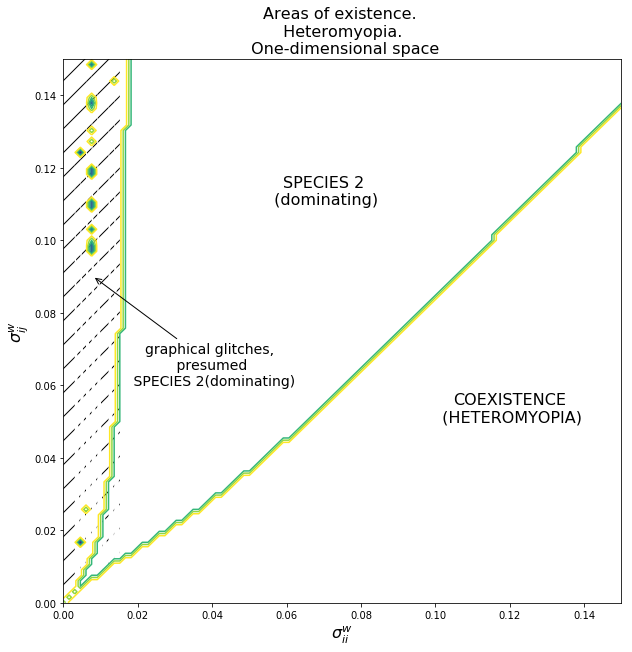
\includegraphics[width=.93\linewidth]{arhm08d1.png}
		\caption{Области сосуществования в описанном пространстве параметров} 
		\label{fig:hmd1:sub2}
	\end{subfigure}
\begin{subfigure}{.5\textwidth}
	\centering
	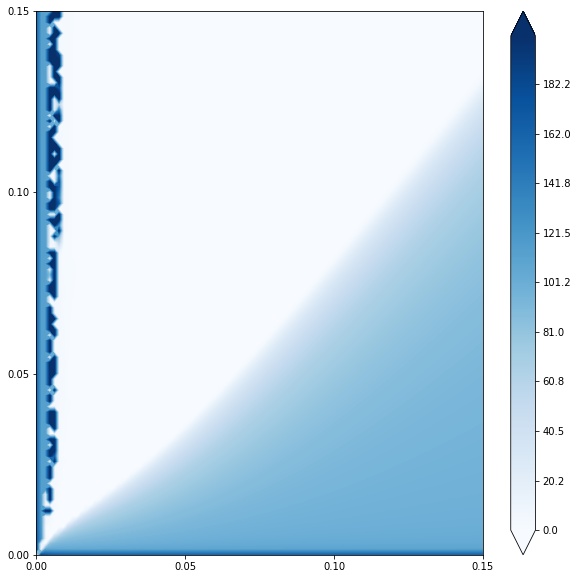
\includegraphics[width=.93\linewidth]{hm_d1_n1.png}
	\caption{Heat map численности первого вида (более сильно распространяющегося) в описанном пространстве параметров}
	\label{fig:hmd1:sub3}
\end{subfigure}%
\begin{subfigure}{.5\textwidth}
	\centering
	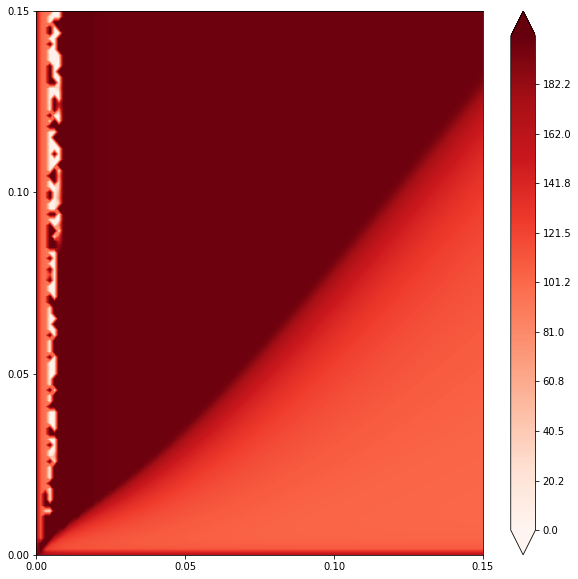
\includegraphics[width=.93\linewidth]{hm_d1_n2.png}
	\caption{Heat map численности первого вида в описанном пространстве параметров} 
	\label{fig:hmd1:sub4}
\end{subfigure}
	\caption{Реализация механизма Heteromyopia в пространстве параметров  $\sigma_{11}^{w}=\sigma_{22}^{w}$ и $\sigma_{12}^{w}=\sigma_{21}^{w}$ в случае \emph{одномерной области обитания}. Оставшиеся параметры выбраны следующим образом: $b_{1}=b_{2}=0.4
		, d_{1}=d_{2}=0.2
		, d'_{11}=d'_{22}=d'_{21}=d'_{12}=0.001,
		\sigma_{1}^{m}=\sigma_{2}^{m}=0.06$. }
	\label{fig:hmd1}
\end{figure*}

\begin{figure*}[ht]
	\centering
	\begin{subfigure}{.5\textwidth}
		\centering
		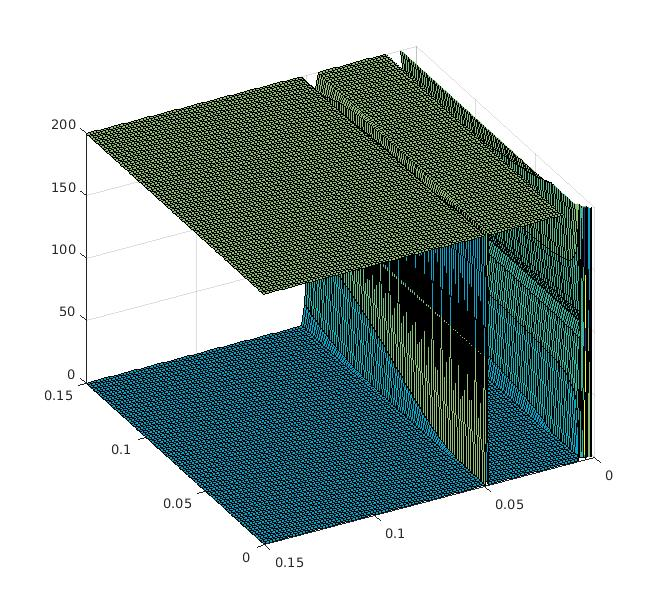
\includegraphics[width=.93\linewidth]{N1N2hm04D2.jpg}
		\caption{Поверхности первых моментов \(N_1\) и \(N_2\) в описанном пространстве параметров}
		\label{fig:hmd2:sub1}
	\end{subfigure}%
	\begin{subfigure}{.5\textwidth}
		\centering
		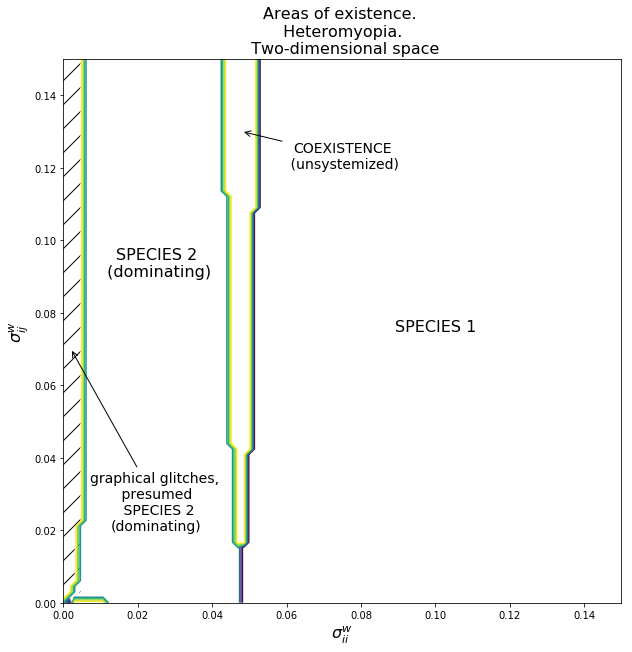
\includegraphics[width=.93\linewidth]{arhm08d2.png}
		\caption{Области сосуществования в описанном пространстве параметров}
		\label{fig:hmd2:sub2}
	\end{subfigure}
\begin{subfigure}{.5\textwidth}
	\centering
	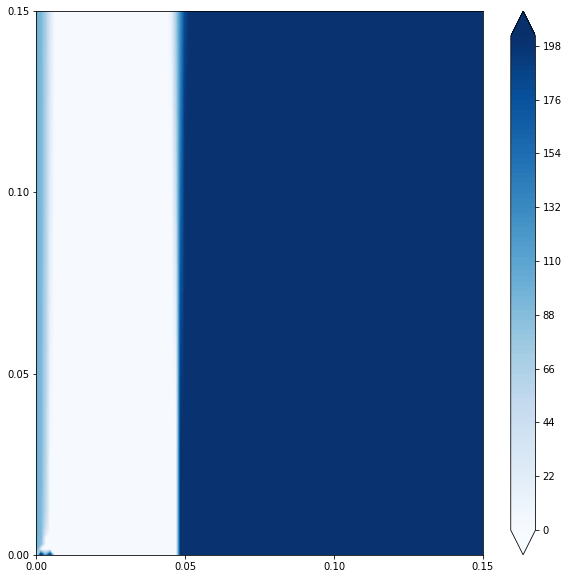
\includegraphics[width=.93\linewidth]{hm_d2_n1.png}
	\caption{Heat map численности первого вида (более сильно распространяющегося) в описанном пространстве параметров}
	\label{fig:hmd2:sub3}
\end{subfigure}%
\begin{subfigure}{.5\textwidth}
	\centering
	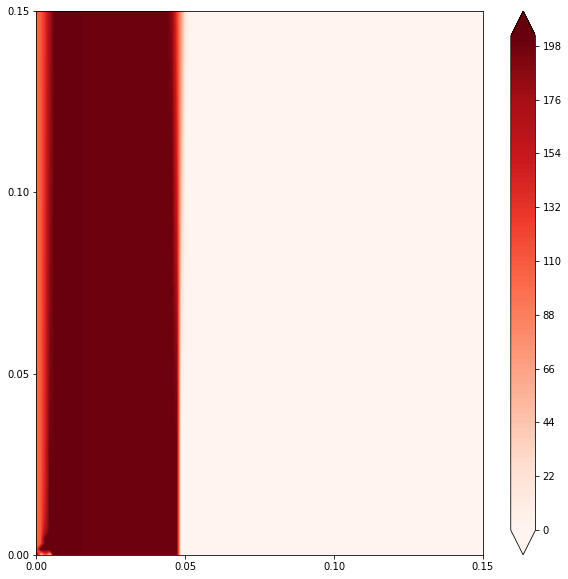
\includegraphics[width=.93\linewidth]{hm_d2_n2.png}
	\caption{Heat map численности первого вида в описанном пространстве параметров}
	\label{fig:hmd2:sub4}
\end{subfigure}
	\caption{Реализация механизма Heteromyopia в пространстве параметров  $\sigma_{11}^{w}=\sigma_{22}^{w}$ и $\sigma_{12}^{w}=\sigma_{21}^{w}$ в случае \emph{двумерной области обитания}. Оставшиеся параметры выбраны следующим образом: $b_{1}=b_{2}=0.4
		, d_{1}=d_{2}=0.2
		, d'_{11}=d'_{22}=d'_{21}=d'_{12}=0.001,
		\sigma_{1}^{m}=\sigma_{2}^{m}=0.06$. }
	\label{fig:hmd2}
\end{figure*}

\begin{figure*}[ht]
	\centering
	\begin{subfigure}{.5\textwidth}
		\centering
		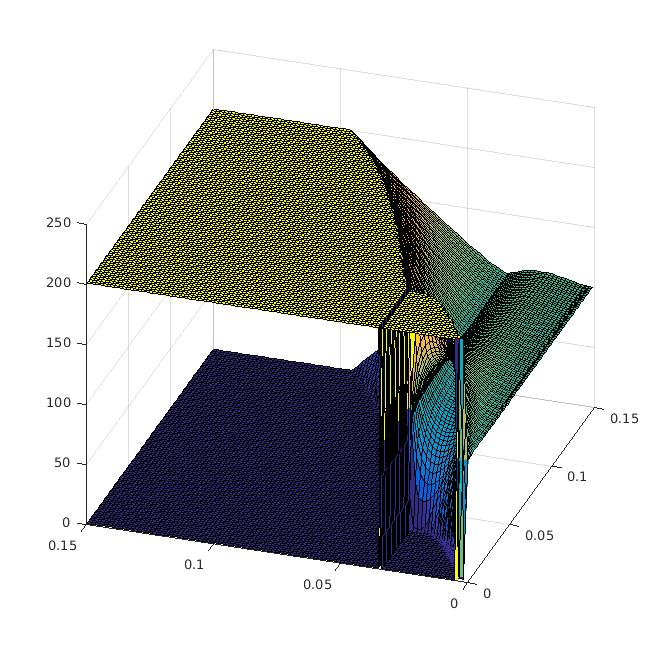
\includegraphics[width=.93\linewidth]{N1N2hm08D3.jpg}
		\caption{Поверхности первых моментов \(N_1\) и \(N_2\) в описанном пространстве параметров}
		\label{fig:hmd3:sub1}
	\end{subfigure}%
	\begin{subfigure}{.5\textwidth}
		\centering
		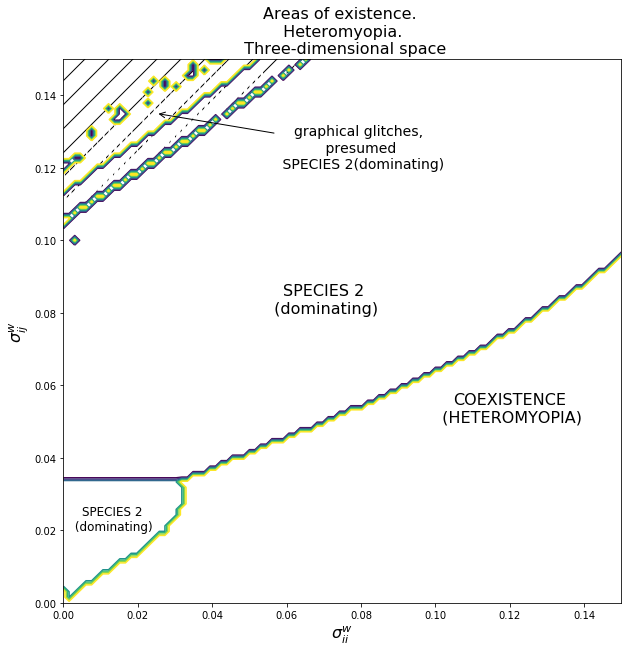
\includegraphics[width=.93\linewidth]{arhm08d3.png}
		\caption{Области сосуществования в описанном пространстве параметров}
		\label{fig:hmd3:sub2}
	\end{subfigure}
	\begin{subfigure}{.5\textwidth}
	\centering
	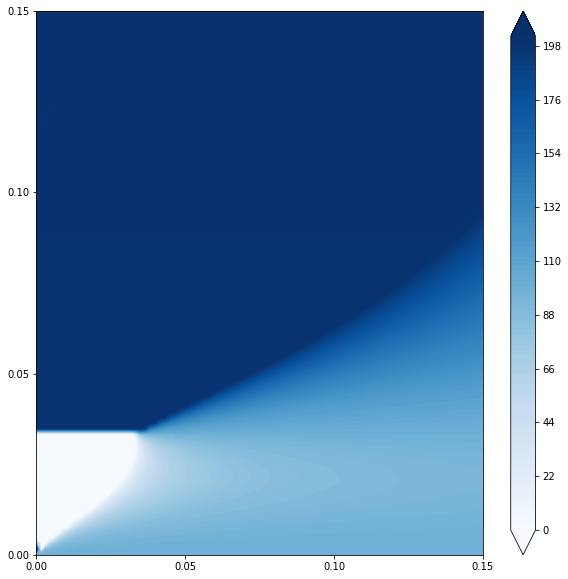
\includegraphics[width=.93\linewidth]{hm_d3_n1.png}
	\caption{Heat map численности первого вида (более сильно распространяющегося) в описанном пространстве параметров}
	\label{fig:hmd3:sub3}
\end{subfigure}%
\begin{subfigure}{.5\textwidth}
	\centering
	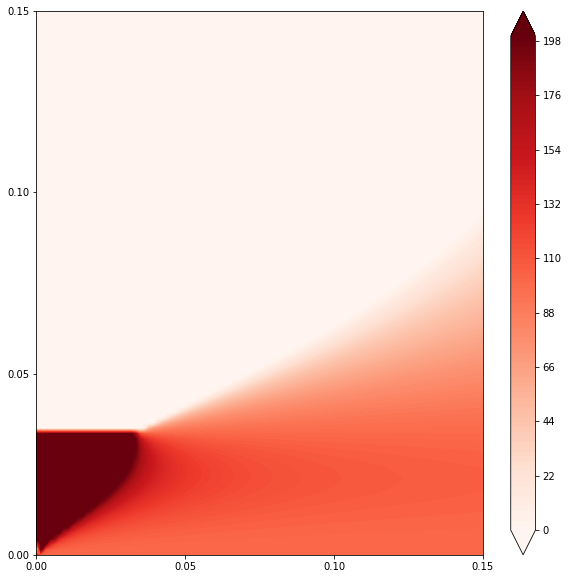
\includegraphics[width=.93\linewidth]{hm_d3_n2.png}
	\caption{Heat map численности первого вида в описанном пространстве параметров}
	\label{fig:hmd3:sub4}
\end{subfigure}
	\caption{Реализация механизма Heteromyopia в пространстве параметров  $\sigma_{11}^{w}=\sigma_{22}^{w}$ и $\sigma_{12}^{w}=\sigma_{21}^{w}$ в случае \emph{трехмерной области обитания}. Оставшиеся параметры выбраны следующим образом: $b_{1}=b_{2}=0.4
		, d_{1}=d_{2}=0.2
		, d'_{11}=d'_{22}=d'_{21}=d'_{12}=0.001,
		\sigma_{1}^{m}=\sigma_{2}^{m}=0.06$. }
	\label{fig:hmd3}
\end{figure*}


\chapter{Заключение}

Подводя итог по всему выше написанному, в рамках данной выпускной квалификационной работы:
\begin{itemize}
	\item	 была изучена модель стационарных пространственно неоднородных сообществ; 
	\item была выведена система нелинейных интегральных уравнений, описывающая стационарное положение системы для широкого семейства замыканий; 
	\item на основе метода рядов Неймана был разработан численный метод для решения возникшей системы с экспоненциальной скоростью сходимости;
	\item для многомерных случаев был разработан математический аппарат, позволяющий свести вычислительную сложность задачи в пространствах больших размерностей к одномерной задаче; в двумерном случае при помощи преобразования Ханкеля; в трехмерном случае при помощи задачи Лапласа на шаре и присоединенных полиномов Лежандра;
	\item разработанный численный метод был применен к изучению влияния размерности внешней среды обитания на предложенные механизмы сосуществования: competition-colonization trade-off и  heteromyopia;
	\item было показано соблюдение принципов механизма competition-colonization trade-off во всех пространствах, с генеральной тенденцией на увеличение численности и конкурентоспособности более дисперсного вида;
	\item было показано соблюдения принципов механизма heteromyopia  в двумерном случае; в остальных пространствах механизм соблюдается.
		
\end{itemize}

Также необходимо указать перечень задач, представляющих интерес для дальнейшего исследования:
\begin{enumerate}
	
\item Проведение биологических симуляций для получения тестовой выборки, на которой можно будет проверить корректность аппроксимации третьего момента и улучшить ее;

\item  Изучение случаев больших размерностей; несмотря на кажущуюся математичность и неприменимость подобных сред обитания в реальной жизни, необходимо отметить, что более чем трехмерные пространства — это классический подход моделирования биоценозов тропических лесов;

\item Изучение работы численного метода и зависимости результатов от ядер другого вида; в частности, рассмотрение ядер конкуренции с сингулярностью в 0, что позволяет моделировать размер индивида, и ядер дисперсии с 0 в 0, что является более корректным биологическим случаем;

\item Получение корректных ядер взаимодействия в модели, согласно имеющимся датасетам о распределении планктона в течениях; центральная сложность данной задачи заключается в том, что получение корректной выборочной функции распределения затруднена наличием градиентов течения и кислорода, влияние которых должно быть учтено при моделировании;

\item Изучение поведение симбионтов (т.е. видов в отрицательной константой конкуренции) с учетом пространственной структуры и наличием внутривидовой конкуренции.

\end{enumerate}

В конце настоящей работы приведем список авторских публикаций, затрагивающих тематику данной работы (без учета курсовых работ) \citeS{nikitin2017netrivialnye57523661,nesterenko2017mekhanizmy57102897,vor2015,vor2016,vmk2015,vmk2016,vmk2017}.